\documentclass{standalone}
\usepackage{amsmath,amssymb}
\usepackage{tikz}
\usetikzlibrary{arrows.meta}

\tikzset{gridline/.style={very thin}}
\tikzset{griddot/.style={circle,fill=black,inner sep=0pt,minimum size=3pt}}
\tikzset{gridline dot/.style={gridline,griddot,draw=none,fill=none}}
\tikzset{gridblue/.style={gridline dot,fill=blue}}
\tikzset{gridred/.style={gridline dot,fill=red}}

\begin{document}
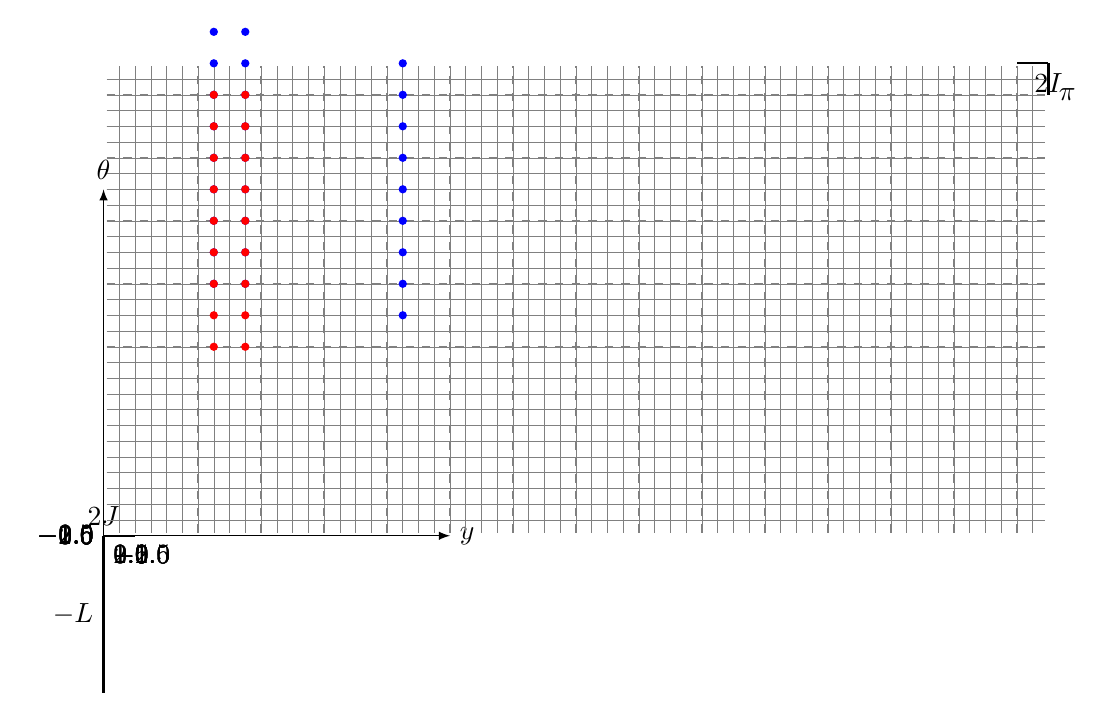
\begin{tikzpicture}[xscale=.4,yscale=.4]
\coordinate (LL) at (-2,-6);
\coordinate (UR) at (28,9);

\draw[thick] (LL) -- node[left] {$-L$} ++(0,-5);
\draw[thick] (UR) |- node[below] {$2I$} ++(-1,0);
\draw[thick] (UR) |- node[right] {$\pi$} ++(0,-1);
\draw[thick] (LL) |- node[above] {$2J$} ++(1,0);

\draw[->,>=latex] (LL)-- ++(0,11) node[above]{$\theta$};
\draw[->,>=latex] (LL)-- ++(11,0) node[right]{$y$};

\foreach \i in {-5,...,5}{
  \node [anchor=north west] at (LL) {\pgfmathparse{\i*(-.5)}
    \pgfmathprintnumber[fixed,fixed zerofill,precision=1]{\pgfmathresult}};
}
\foreach \i in {-5,...,5}{
  \node [anchor=east] at (LL) {\pgfmathparse{\i*(.5)}
    \pgfmathprintnumber[fixed,fixed zerofill,precision=1]{\pgfmathresult}};
}

\draw[gray,help lines] 
    ([shift={(.1,.1)}]LL) grid[step=.5] ([shift={(-.1,-.1)}]UR);
\draw[gray,dashed] 
    ([shift={(.1,.1)}]LL) grid[step=1] ([shift={(-.1,-.1)}]UR);

\foreach \x in {1,...,2}{
  \foreach \y in {1,...,9}{
    \node [gridblue] at (\x+.5,\y+1){
    };
    \node [gridred] at (\x+.5,\y-1){
    };
  }
}

\foreach \y in {1,...,9}{
  \node [gridblue] at (7+.5,\y){
    };
}

\end{tikzpicture}
\end{document}